\subsubsection{The van Keken thermochemical composition benchmark}
\label{sec:benchmark-van-keken}

\textit{This section is a co-production of Cedric Thieulot, Juliane Dannberg,
Timo Heister and Wolfgang Bangerth with an extension to this benchmark provided by the Virginia Tech Department of Geosciences class ``Geodynamics and ASPECT'' co-taught by Scott King and D.~Sarah Stamps.}

One of the most widely used benchmarks for mantle convection codes is the
isoviscous Rayleigh-Taylor case (``case 1a'') published by van Keken \textit{et
al.} in \cite{KKSCND97}.
The benchmark considers a 2d situation where a lighter fluid underlies a heavier
one with a non-horizontal interface between the two of them. This unstable
layering causes the lighter fluid to start rising at the point where the
interface is highest. Fig.~\ref{fig:vk-1} shows a time series of images to
illustrate this.

\begin{figure}
  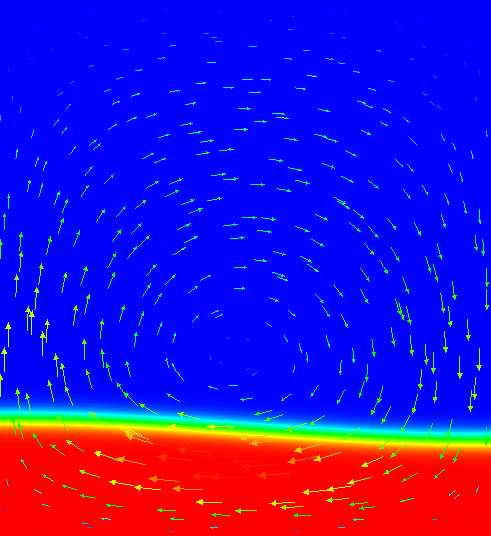
\includegraphics[width=0.23\textwidth]{cookbooks/benchmarks/van-keken/doc/movie0000.png}
  \hfill
  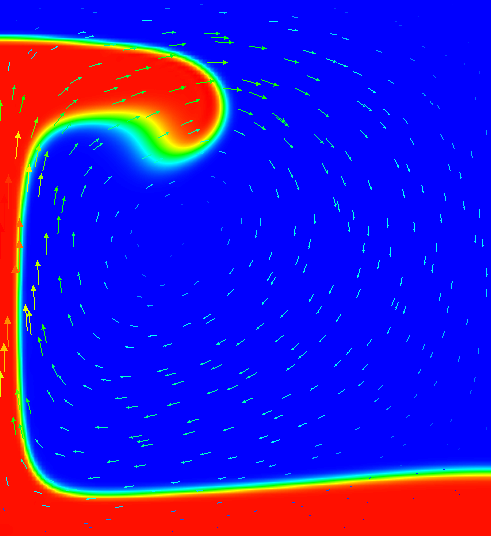
\includegraphics[width=0.23\textwidth]{cookbooks/benchmarks/van-keken/doc/movie0003.png}
  \hfill
  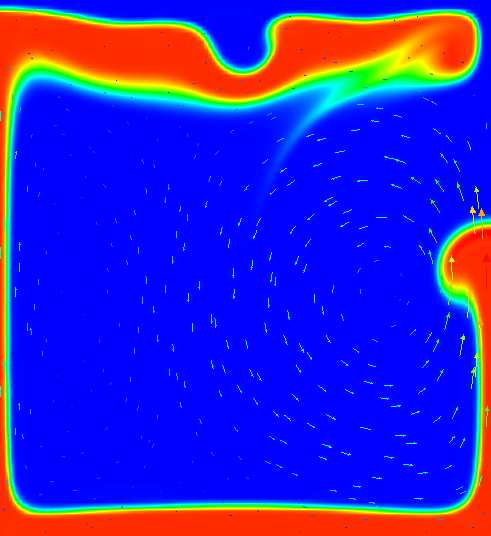
\includegraphics[width=0.23\textwidth]{cookbooks/benchmarks/van-keken/doc/movie0009.png}
  \hfill
  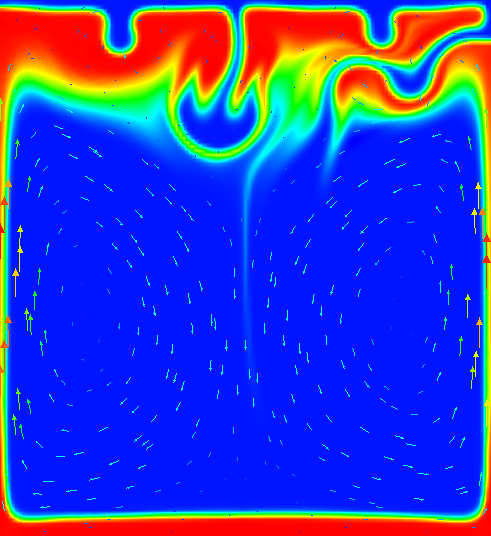
\includegraphics[width=0.23\textwidth]{cookbooks/benchmarks/van-keken/doc/movie0018.png}
  \caption{\it Van Keken benchmark (using a smoothed out interface, see the main
  text):
  Compositional field at times $t=0, 300, 900, 1800$.}
  \label{fig:vk-1}
\end{figure}


Although van Keken's paper title suggests that the paper is really about
thermochemical convection, the part we examine here can equally be considered as
thermal or chemical convection; all that is necessary is that we describe the
fluid's density. We can do that by using an inhomogeneous initial
temperature field, or an inhomogeneous initial composition field. We will use the
input file in \url{cookbooks/van-keken/van-keken-discontinuous.prm} as input, the central
piece of which is as follows (go to the actual input file
to see the remainder of the input parameters):

\lstinputlisting[language=prmfile]{cookbooks/benchmarks/van-keken/doc/main.part.prm.out}

The first part of this selects the \texttt{simple} material model and sets the
thermal expansion to zero (resulting in a density that does not depend on the
temperature, making the temperature a passively advected field) and instead
makes the density depend on the first compositional field. The second section
prescribes that the first compositional field's
initial conditions are 0 above a line describes by a cosine and 1 below it.
Because the dependence of the density on the compositional field is negative,
this means that a lighter fluid underlies a heavier one.

The dynamics of the resulting flow have already been shown in
Fig.~\ref{fig:vk-1}. The measure commonly considered in papers comparing
different methods is the root mean square of the velocity, which we can get
using the following block in the input file (the actual input file also enables
other postprocessors):

\lstinputlisting[language=prmfile]{cookbooks/benchmarks/van-keken/doc/postprocess.part.prm.out}

Using this, we can plot the evolution of the fluid's average velocity over time,
as shown in the left panel of Fig.~\ref{fig:vk-2}. Looking at this graph, we
find that both the timing and the height of the first peak is already
well converged on a simple
$32\times 32$ mesh (5 global refinements) and is very consistent (to better
than 1\% accuracy) with the results in the van Keken paper.

\begin{figure}
  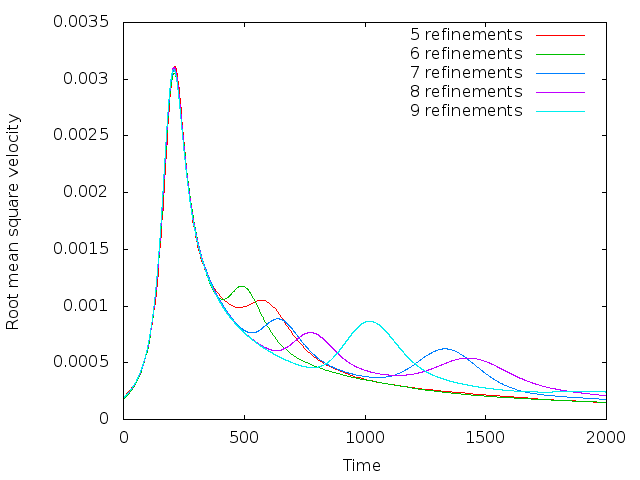
\includegraphics[width=0.48\textwidth]{cookbooks/benchmarks/van-keken/doc/velocity-discontinuous.png}
  \hfill
  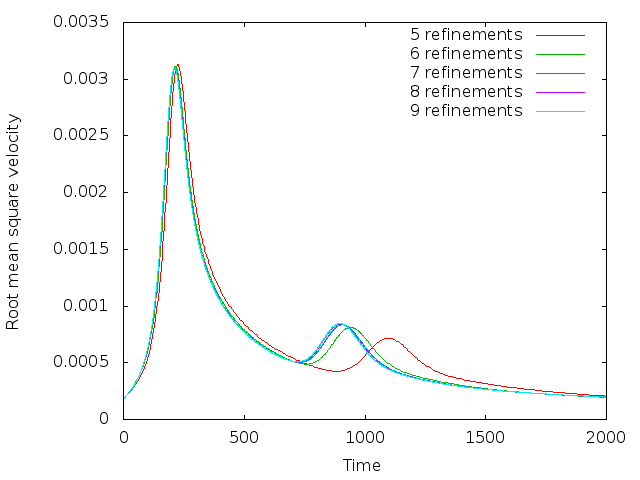
\includegraphics[width=0.48\textwidth]{cookbooks/benchmarks/van-keken/doc/velocity-smooth.png}
  \caption{\it Van Keken benchmark with discontinuous (left) and smoothed,
  continuous (right) initial conditions for the compositional field:
  Evolution of the root mean square velocity $\left(\frac 1{|\Omega|}\int_\Omega |\mathbf u(\mathbf x,t)|^2 \;
  \text{d}x\right)^{1/2}$ as a function of time for different numbers of global mesh
  refinements. 5 global refinements correspond to a $32\times 32$ mesh, 9
  refinements to a $512\times 512$ mesh.}
  \label{fig:vk-2}
\end{figure}

That said, it is startling that the second peak does not appear to converge
despite the fact that the various codes compared in \cite{KKSCND97} show good
agreement in this comparison. Tracking down the cause for this proved to be a
lesson in benchmark design; in hindsight, it may also explain why van Keken
\textit{et al.} stated presciently in their abstract that ``\textit{\ldots good
agreement is found for the initial rise of the unstable lower layer; however, the timing
  and location of the later smaller-scale instabilities may differ between
  methods.}''
To understand what is happening here, note that the first peak in these plots
corresponds to the plume that rises along the left edge of the domain and whose
evolution is primarily determined by the large-scale shape of the initial
interface (i.e., the cosine used to describe the initial conditions in the
input file). This is a first order deterministic effect, and is obviously
resolved already on the coarsest mesh shown used. The second peak corresponds to
the plume that rises along the right edge, and its origin along the interface is
much harder to trace -- its position and the timing when it starts to rise is
certainly not obvious from the initial location of the interface. Now recall
that we are using a finite element field using continuous shape functions for
the composition that determines the density differences that drive the flow. But
this interface is neither aligned with the mesh, nor can a discontinuous
function be represented by continuous shape functions to begin with. In other
words, we may \textit{input} the initial conditions as a discontinuous functions
of zero and one in the parameter file, but the initial conditions used in the
program are in fact different: they are the \textit{interpolated} values of this
discontinuous function on a finite element mesh. This is shown in
Fig.~\ref{fig:vk-3}. It is obvious that these initial conditions agree on the
large scale (the determinant of the first plume), but not in the steps that may
(and do, in fact) determine when and where the second plume will rise. The
evolution of the resulting compositional field is shown in Fig.~\ref{fig:vk-4}
and it is obvious that the second, smaller plume starts to rise from a
completely different location -- no wonder the second peak in the root mean
square velocity plot is in a different location and with different height!

\begin{figure}
  \centering
  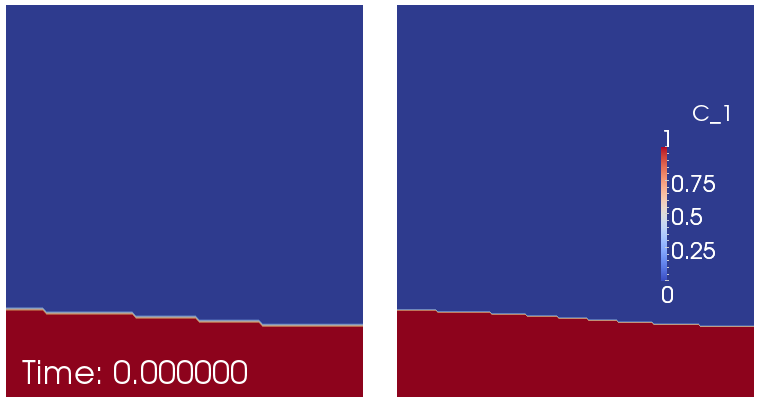
\includegraphics[width=0.7\textwidth]{cookbooks/benchmarks/van-keken/doc/mesh-comparison-initial-conditions.png}
  \caption{\it Van Keken benchmark with discontinuous initial conditions for the
  compositional field:
  Initial compositional field interpolated onto a $32\times 32$ (left) and
  $64\times 64$ finite element mesh (right).}
  \label{fig:vk-3}
\end{figure}

\begin{figure}
  \centering
  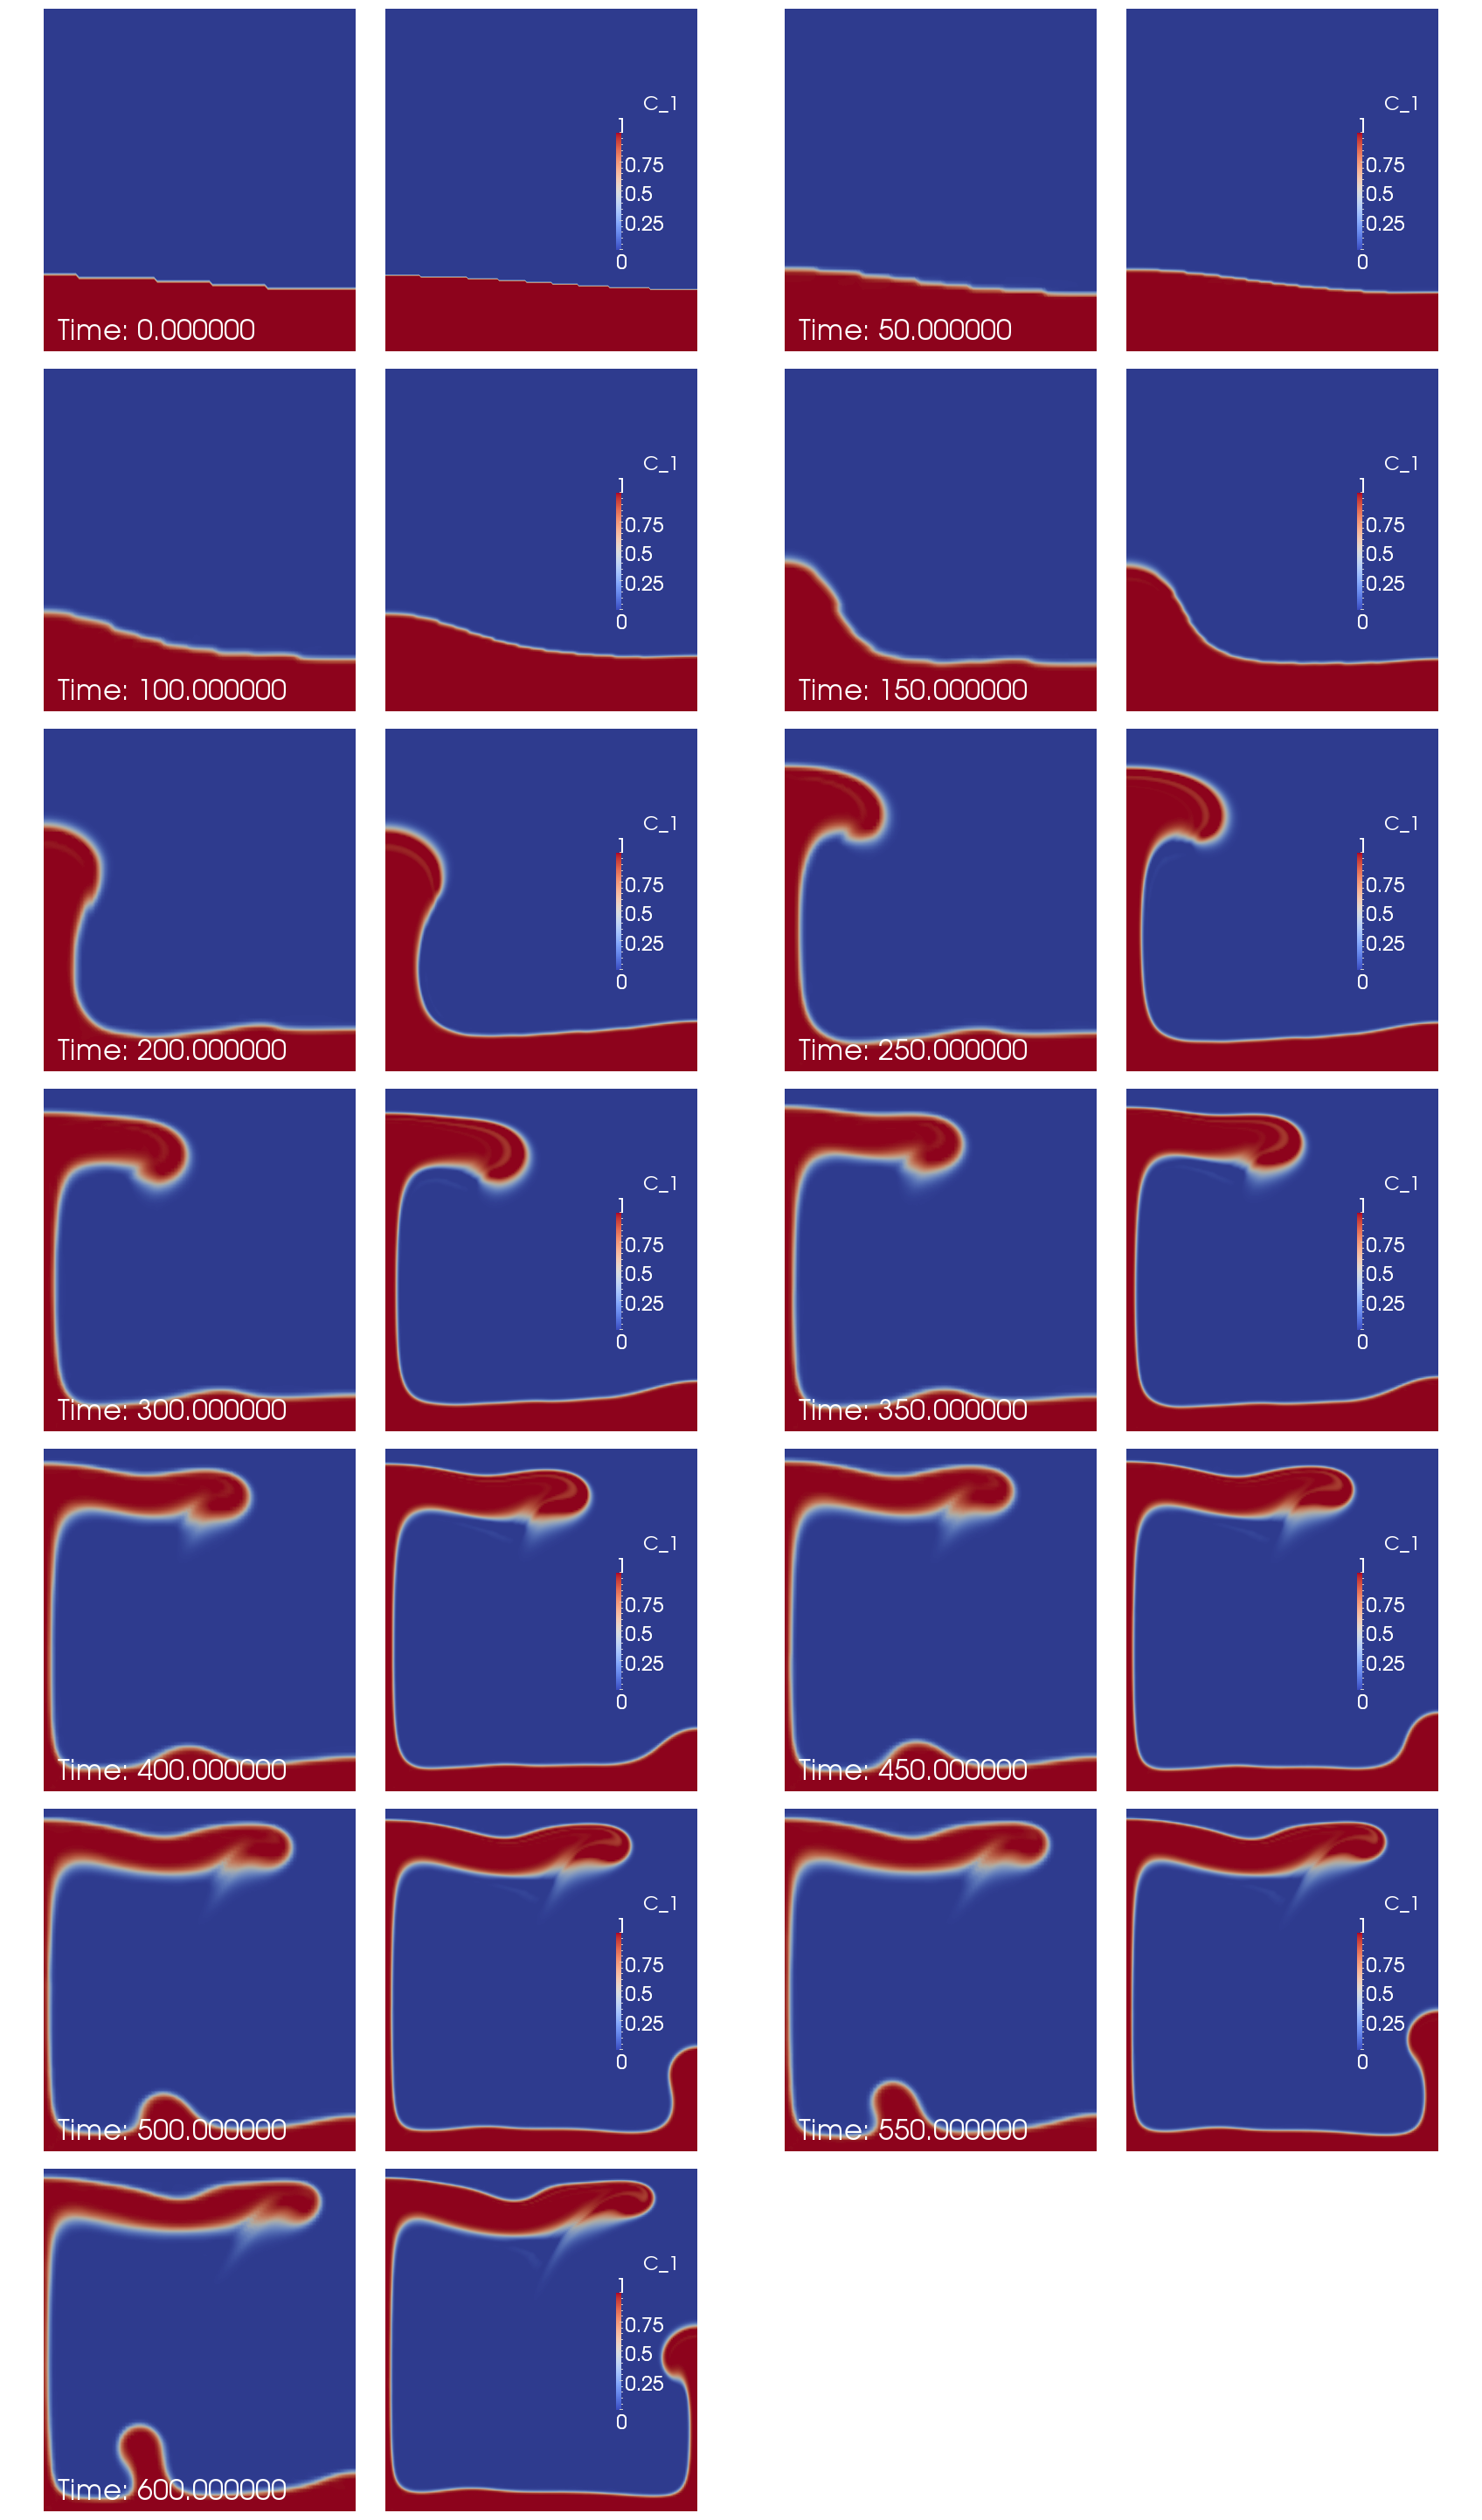
\includegraphics[height=0.8\textheight]{cookbooks/benchmarks/van-keken/doc/mesh-comparison.png}
  \caption{\it Van Keken benchmark with discontinuous initial conditions for the
  compositional field:
  Evolution of the compositional field over time on a $32\times 32$ (first and
  third column; left to right and top to bottom) and $64\times 64$ finite
  element mesh (second and fourth column). Pictures next to each other
  illustrate how critically the rise of the second plume depends on
  the mesh resolution, starting at around time $t=350$.}
  \label{fig:vk-4}
\end{figure}

The conclusion one can draw from this is that if the outcome of a computational
experiment depends so critically on very small details like the steps of an
initial condition, then it's probably not a particularly good measure to look at
in a benchmark. That said, the benchmark is what it is, and so we should try to
come up with ways to look at the benchmark in a way that allows us to reproduce
what van Keken \textit{et al.} had agreed upon. To this end, note that the codes
compared in that paper use all sorts of different methods, and one can certainly
agree on the fact that these methods are not identical on small length scales.
One approach to make the setup more mesh-independent is to replace the original
discontinuous initial condition with a smoothed out version; of course, we can
still not represent it exactly on any given mesh, but we can at least get closer
to it than for discontinuous variables. Consequently, let us use the following
initial conditions instead (see also the file
\url{cookbooks/van-keken/van-keken-smooth.prm}):
\lstinputlisting[language=prmfile]{cookbooks/benchmarks/van-keken/doc/smooth.part.prm.out}


This replaces the discontinuous initial conditions with a smoothed out version
with a half width of around 0.01. Using this, the root mean square plot now
looks as shown in the right panel of Fig.~\ref{fig:vk-2}. Here, the second peak
also converges quickly, as hoped for.

The exact location and height of the two peaks is in good agreement with those
given in the paper by van Keken \textit{et al.}, but not exactly where desired
(the error is within a couple of per cent for the first peak, and probably
better for the second, for both the timing and height of the peaks).
This has to do with the fact that they depend on the exact size of the smoothing
parameter (the division by 0.02 in the formula for the smoothed initial
condition). However, for more exact results, one can choose
this half width parameter proportional to the mesh size and thereby get more
accurate results. The point of the section was to demonstrate the reason
for the lack of convergence.

\paragraph*{Extension to an adaptive smoothing lengthscale.}
In this section we extend the van Keken cookbook following up the work previously completed by Cedric Thieulot, Juliane Dannberg,
Timo Heister and Wolfgang Bangerth.  \textit{This section contributed by Grant Euen, Tahiry Rajaonarison, and Shangxin Liu as part of the Geodynamics and ASPECT class at Virginia Tech.}

As already mentioned above, using a half width parameter proportional to the mesh size allows for more accurate results.  We test the effect of the half width size of the smoothed discontinuity by changing the smoothing parameter to values proportional to the mesh size.  In the formula for the smoothed initial conditions, this parameter is the division by 0.02.  We use 7 global refinements because the root mean square velocity converges at greater resolution while keeping average runtime around 5 to 25 minutes.  These runtimes were produced by the BlueRidge cluster of the Advanced Research Computing (ARC) program at Virginia Tech.  BlueRidge is a 408-node Cray CS-300 cluster; each node outfitted with two octa-core Intel Sandy Bridge CPUs and 64 GB of memory.  Average runtimes for global refinements 5 through 10 using one node can be seen in Table~\ref{tab:runtime-table}.  For 7 global refinements (128$\times$128 mesh size), the size of the mesh is 0.0078 corresponding to a half width parameter of 0.0039.  The smooth model allows for much better convergence of the secondary plumes, although they are still more scattered than the primary plumes.

\begin{table}[tb]
        \center
        \begin{tabular}{|c|cccc|}
                \hline
                Global & \multicolumn{4}{c}{Number of Processors} \\
                Refinements & 4 & 8 & 12 & 16
                \\ \hline
                5 & 28.1 seconds & 19.8 seconds & 19.6 seconds & 17.1 seconds \\
                6 & 3.07 minutes & 1.95 minutes & 1.49 minutes & 1.21 minutes \\
                7 & 23.33 minutes & 13.92 minutes & 9.87 minutes & 7.33 minutes \\
                8 & 3.08 hours & 1.83 hours & 1.30 hours & 56.33 minutes \\
                9 & 1.03 days & 15.39 hours & 10.44 hours & 7.53 hours \\
                10 & More than 6 days & More than 6 days & 3.39 days & 2.56 days \\ \hline
        \end{tabular}
        \caption{\it Average runtimes for the van Keken Benchmark with smoothed initial conditions.  These times are for the entire computation, a final time step number of 2000.  All of these tests were run using ASPECT version 1.3 in release mode, and used different numbers of processors on one node on the BlueRidge cluster of ARC at Virginia Tech.}
        \label{tab:runtime-table}
\end{table}

This convergence is due to changing the smoothing parameter, which controls how much of the problem is smoothed over.  As the parameter is increased the smoothed boundary grows; as the smoothed boundary shrinks it becomes sharper until the original discontinuous behavior is revealed.  As the boundary grows, the two distinct layers eventually become one large, transitioning layer.  These effects can be seen in Fig.~\ref{fig:vk-5}.  The overall effect is that the secondary rise is at different times based on these conditions.  In general, as the smoothing parameter is decreased the smoothed boundary shrinks, and the plumes rise more quickly.  As it is increased the boundary grows, and the plumes rise more slowly.  This trend can be used to force a more accurate convergence from the secondary plumes.

\begin{figure}
        \centering
        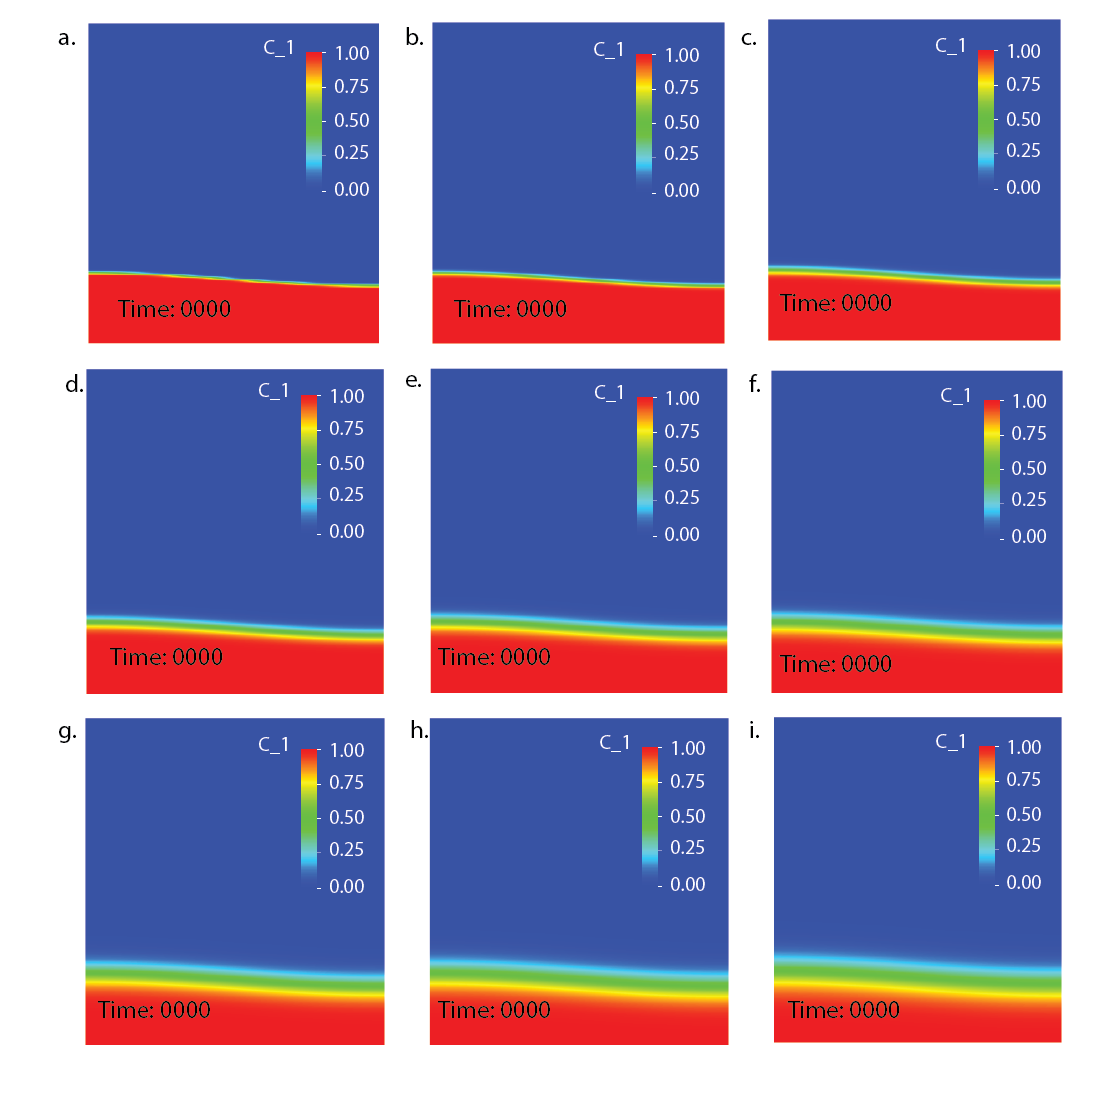
\includegraphics[width=0.6\textwidth]{cookbooks/benchmarks/van-keken/doc/smoothing-parameter.png}
        \caption{\it Van Keken Benchmark using smoothed out interface at 7 global refinements: compositional field at time $t=0$ using smoothing parameter size: a) 0.0039, b) 0.0078, c) 0.0156, d) 0.0234, e) 0.0312, f) 0.0390, g) 0.0468, h) 0.0546, i) 0.0624.}
        \label{fig:vk-5}
\end{figure}

The evolution in time of the resulting compositional fields (Fig.~\ref{fig:vk-6}) shows that the first peak converges as the smoothed interface decreases. There is a good agreement for the first peak for all smoothing parameters.  As the width of the discontinuity increases, the second peak rises more slowly and later in the run.

\begin{figure}
        \centering
        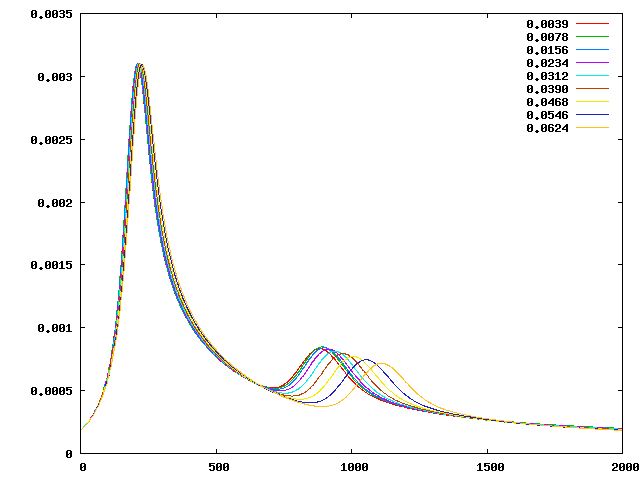
\includegraphics[width=0.4\textwidth]{cookbooks/benchmarks/van-keken/doc/smoothing-parameter-velocity.png}
        \caption{\it Van Keken benchmark with smoothed initial conditions for the compositional field using 7 global refinements for different smoothing parameters.  Number of the time step is shown on the $x$-axis, while root mean square velocity is shown on the $y$-axis.}
        \label{fig:vk-6}
\end{figure}

Now let us further add a two-layer viscosity model to the domain. This is done to recreate the two nonisoviscous Rayleigh-Taylor instability cases (``cases 1b and 1c'') published in van Keken \textit{et al.} in \cite{KKSCND97}.  Let's assume the viscosity value of the upper, heavier layer is $\eta_{t}$ and the viscosity value of the lower, lighter layer is $\eta_{b}$. Based on the initial constant viscosity value 1$\times10^{2}$ \si{Pa.s}, we set the viscosity proportion $\frac{\eta_{t}}{\eta_{b}}=0.1, 0.01$, meaning the viscosity of the upper, heavier layer is still 1$\times10^{2}$ \si{Pa.s}, but the viscosity of the lower, lighter layer is now either 10 or 1 \si{Pa.s}, respectively. The viscosity profiles of the discontinuous and smooth models are shown in Fig.~\ref{fig:vk-7}.

\begin{figure}
        \centering
        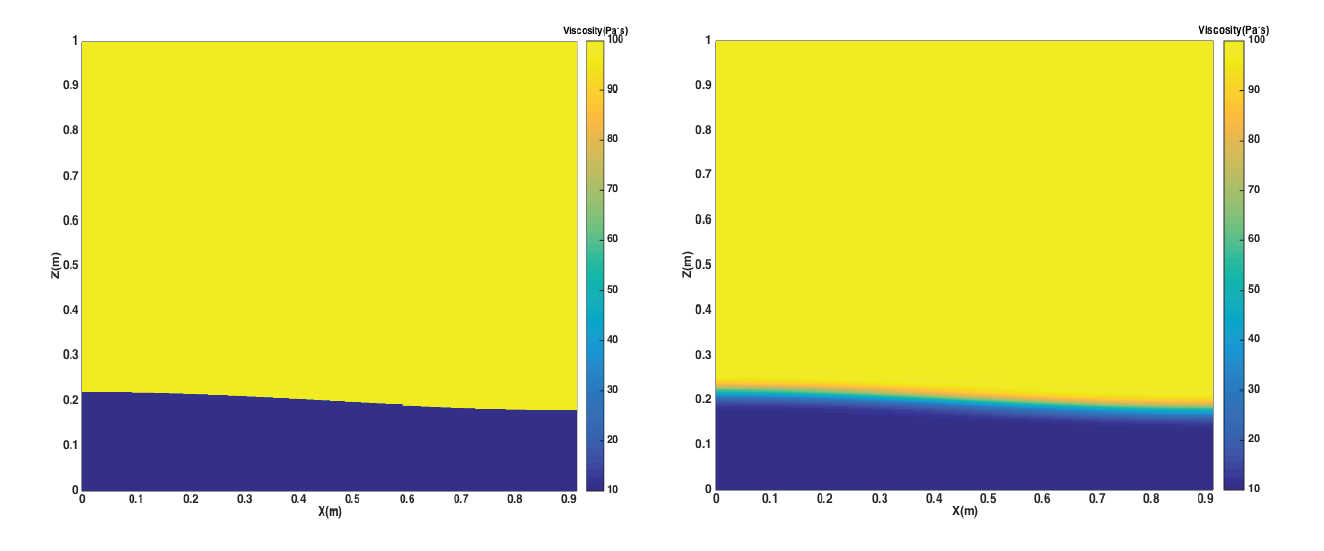
\includegraphics[width=0.7\textwidth]{cookbooks/benchmarks/van-keken/doc/contrast_viscosity.png}
        \caption{\it Van Keken benchmark using different-viscosity layers. The left image is the discontinuous case, while right is the smooth.  Both are shown at $t=0$.}
        \label{fig:vk-7}
\end{figure}

For both cases, discontinuous and smooth, and both viscosity proportions, 0.1 and 0.01, the results are shown at the end time step number, $t=2000$, in Fig.~\ref{fig:vk-8}.  This was generated using the original input parameter file, running the cases with 8 global refinements, and also adding the two-layer viscosity model.

\begin{figure}
        \centering
        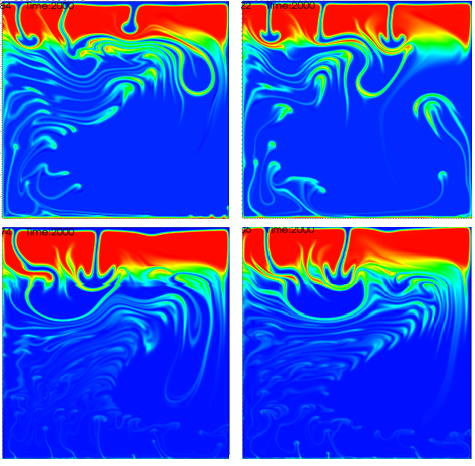
\includegraphics[width=0.5\textwidth]{cookbooks/benchmarks/van-keken/doc/2viscosities-final.png}
        \caption{\it Van Keken benchmark two-layer viscosity model at final time step number, $t=2000$. These images show layers of different compositions and viscosities. Discontinuous cases are the left images, smooth cases are the right. The upper images are $\frac{\eta_{t}}{\eta_{b}}=0.1$, and the lower are $\frac{\eta_{t}}{\eta_{b}}=0.01$.}
        \label{fig:vk-8}
\end{figure}

Compared to the results of the models using constant viscosity throughout the domain, the plumes rise faster when adding the two-layer viscosity. Also, the larger the viscosity difference is the earlier the plumes appear, and the faster their ascent. To further reveal the effect of the two-layer viscosity model, we also plot the evolution of the fluids' root mean square velocity over time, as shown in Fig.~\ref{fig:vk-9}.

\begin{figure}
        \centering
        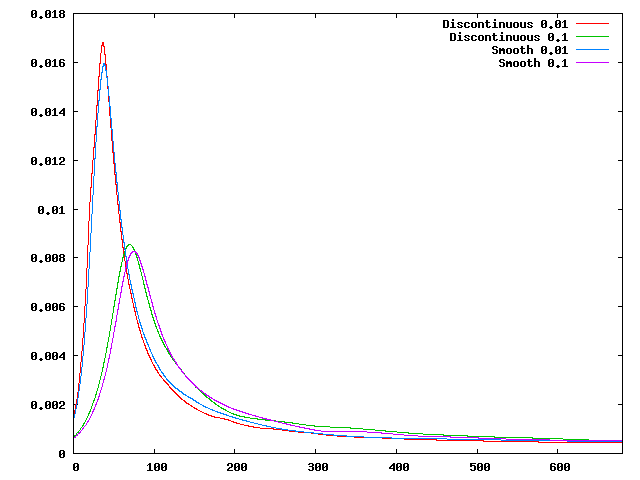
\includegraphics[width=0.4\textwidth]{cookbooks/benchmarks/van-keken/doc/2viscosities-velocity.png}
        \caption{\it Van Keken benchmark: Evolution of the root mean square velocity as a function of time for different viscosity contrast proportions (0.1/0.01) for both discontinuous and smooth models.}
        \label{fig:vk-9}
\end{figure}

We can observe that when the two-layer viscosity model is added, there is only one apparent peak for each case. The first peaks of the 0.01 viscosity contrast tests appear earlier and are larger in magnitude than those of 0.1 viscosity contrast tests.  There are no secondary plumes and the whole system tends to reach stability after around 500 time steps.
